% =====================================================================
% "Context Compounds, Capability Does Not" — Conductor experience report.
% Target: ICSE 2027 SEIP. SINGLE HUMAN AUTHOR (Kyle Fox); the fleet's role is
% disclosed in the "Disclosure: Use of Generative AI" section, not as a byline
% (ACM/IEEE policy forbids an AI author). All counts carry one as-of stamp: 2026-07-31.
%
% Build:  pdflatex conductor-paper && bibtex conductor-paper && pdflatex x2
% Needs:  IEEEtran.cls + IEEEtran.bst + references.bib (in this dir).
% =====================================================================
\documentclass[10pt,conference]{IEEEtran}   % ICSE SEIP format: 10pt conference, NO compsoc
\IEEEoverridecommandlockouts

\usepackage{cite}
\usepackage{amsmath,amssymb}
\usepackage{graphicx}
\usepackage{booktabs}
\usepackage{tikz}
\usetikzlibrary{arrows.meta,positioning,fit,backgrounds}
\usepackage{url}
\usepackage[T1]{fontenc}
\usepackage[utf8]{inputenc}
\usepackage{textcomp}   % for \texttimes etc.

\begin{document}

% ---- TITLE + AUTHORS -------------------------------------------------
% AUTHORSHIP (revised per external review, 2026-07-27): SINGLE HUMAN AUTHOR. ACM/IEEE policy
% (binding for the SEIP target) forbids a generative-AI system as an author — listing one is an
% administrative DESK-REJECT. The fleet's contribution is instead DISCLOSED precisely (see the
% "Disclosure: Use of Generative AI" section) + acknowledged. For a paper whose subject IS agent
% co-authorship, an explicit division-of-labour disclosure is stronger than a byline anyway.
\title{Context Compounds, Capability Does Not:\\
       An Experience Report on a Persistent Multi-Agent System}

\author{\IEEEauthorblockN{Kyle Fox}
\IEEEauthorblockA{Independent Researcher\\
Austin, Texas, USA\\
Email: \textit{[to fill at submission]}}}

\maketitle

% ---- ABSTRACT (drafted from draft-v4; trim to venue word limit if needed) ----
\begin{abstract}
Conductor is a fleet of persistent, memory-divergent agent sessions --- one base model, durable
per-session context, a shared append-only bus, and a human gating only irreversible actions. Over a
months-long live deployment the sessions co-designed and hardened their own coordination substrate in
vivo under adversarial peer review, closing roughly twenty named failure modes, and caught one
another's defects from divergent empirical vantages. We report two things the deployment supports. The
first is a reusable taxonomy of \emph{silent} coordination defects --- failures that return a
plausible answer rather than an error, and so survive every gate that checks for errors --- with a
distinct remedy per class, because a single generic discipline sails past most of them. The second is
that peer sessions catch defects their author and the human miss, evidenced from the timestamped
record rather than recalled. We also report, at length, what the deployment could \emph{not}
establish. We set out to test whether accumulated context makes a session more capable on task
$N{+}1$; an earlier version of this paper reported that it does not, and we withdraw that negative.
The ablation behind it never manipulated the construct it named, and no arm of any task ever failed,
so its falsifier was unreachable. The pre-registered replacement cannot be fielded here at all: a
fleet running one session per repository has no second session with the same history, so it cannot
furnish a within-domain control arm for any claim about accumulated context --- a property of the
architecture, not of the hypothesis. Two further claims are withdrawn on defects found by outside
review after we considered the paper ready, both in the direction that flattered it, and we report
them as specimens of our own taxonomy: a longitudinal human-attention trend whose instrument drops
records at a rate that rises with fleet size --- the same direction as the claimed effect --- and a
pre-registered baseline whose target turned out to be one day old, measuring authorship recency
rather than accumulated context. The practitioner consequences we still stand behind: commit
everything that must stay true to the carrier any fresh session can read; give silent-failure classes
named remedies rather than a general injunction to be careful; and treat a peer with a different
vantage as an instrument, not a courtesy.
\end{abstract}

\begin{IEEEkeywords}
LLM agents, multi-agent systems, agent memory, coordination substrate, human-in-the-loop,
experience report, ablation study, self-adaptive systems
\end{IEEEkeywords}

% =====================================================================
% BODY --- converted from draft-v5.md. Each \section maps 1:1 to a draft-v5 section.
% =====================================================================

\section{Introduction and Contributions}
\IEEEPARstart{T}{he} prevailing agentic pattern is an orchestrator dispatching to
stateless workers --- reproducible, but \emph{permanently at task 1}: no carried expertise,
no division of labour, no shared context. Conductor inverts the premise: long-lived sessions
with divergent memories talk to each other and build their own coordination substrate.

This paper reports what that deployment established, and it is narrower than what we set out to
show. Two contributions survive contact with their own evidence:

\begin{enumerate}
\item \textbf{A reusable taxonomy of silent coordination defects}, derived from the failure modes
  closed in a live multi-agent substrate (\S V-B). Several are ablation-structured --- disable the
  mechanism and the failure returns --- and at least one ablated in operation. The taxonomy's value
  is that a single discipline (``just replicate,'' ``just tag'') sails past most of its classes,
  each of which has a distinct remedy.
\item \textbf{Cross-context peer review catches defects that individual sessions and the human
  miss} (\S V-C), evidenced from the timestamped record: A ships at $t_0$, B refutes at $t_1$, both
  attested. This is the claim the deployment supports best, and it is the one we were least
  expecting to lead with.
\end{enumerate}

The system and the method that produced them --- in-vivo adversarial co-design under
reversibility-calibrated HITL, where primitives were \emph{provoked by silent-loss failures} rather
than designed up front, and a human's approval is scoped to \emph{irreversibility} (commits are
free; pushes, and anything outliving the session, are gated) --- are reported as the \emph{setting},
not as a validated result. We never ran the method against an engineer specifying the primitives up
front, so we claim only that it is replicable, has a stated mechanism, and demonstrably produced a
working substrate.

This is an experience report and we ask to be judged at that bar: the contribution is what a
months-long real deployment reveals. We claim neither statistical generality ($N{=}1$ deployment)
nor emergent intelligence.

\emph{What we cannot claim, stated first because an earlier draft claimed it.} We set out to show
that capability compounds --- that a context-carrying session solves what a fresh one cannot. It
does not appear here, for two separate reasons, and neither is a null result. Our original ablation
never manipulated the construct it named, and no arm of any task ever failed, so the falsifier was
unreachable (\S V-D). The pre-registered replacement then could not be fielded at all: this fleet
runs one session per repository, so the only domain able to supply six live context-carrying arms is
the one the authors wrote (\S VIII). Per that pre-registration's committed interpretation, inability
to construct a discriminating task is reported as a \emph{measurement-capability limit of the
deployment} and never as evidence for the negative.

\subsection{What each contribution rests on, and what would falsify it}
The two contributions are not epistemically equal, and neither is a controlled result.

\textbf{The taxonomy (contribution~1)} rests on failure modes we closed and can point at: the fix
commits exist, several are ablation-structured, and the classes were derived from the defects rather
than imposed on them. \emph{Falsifier:} the taxonomy weakens if its classes collapse into one another
under a larger corpus, or if a single generic discipline --- replicate everything, tag everything ---
would have caught the same defects without the classification. We report the classes we could not
merge; a reader who can merge them has refuted this.

\textbf{Peer catching (contribution~2)} rests on the timestamped record: A ships at $t_0$, B refutes
at $t_1$. \emph{Falsifier:} it weakens if the catches would have been made as readily by ordinary
single-author review, or if the peer's advantage is really access rather than vantage --- B seeing a
file A could not. We separate those two claims explicitly in \S V-C because an earlier draft
conflated them. \emph{And a limit we cannot engineer away:} the fleet's primary record is an
append-only message log held outside the public repository, so catches are attested by us and
verifiable by a reader only through the curated extract we publish. The classification is checkable;
the completeness of the underlying log is not.

\textbf{The method} has no controlled evidence at all and we do not claim it is superior to up-front
design. \emph{Falsifier:} the method claim weakens if the primitives it converged on are worse than a
competent engineer's up-front design --- a comparison we did not run.

\emph{A note on the direction of our own errors.} Every correction forced on this paper by review
moved a claim \emph{down}: a negative we called solid was unsound, a signal we called supporting was
confounded, and two catch attributions were wrong in the flattering direction. We have found no
instance of review moving one of our claims up. A reader should weight the remaining claims
accordingly, and we say so here rather than in a closing threats section, where it would arrive too
late to be used.

\begin{table}[t]
\centering\footnotesize
\caption{Human touch per active project (\texttt{history.jsonl}). Jan/Mar (1 and 7 prompts) are
omitted; April, the substrate's build-out month, is shown but excluded from the shape claim as
bootstrap-heavy. Three buckets cannot
establish a trend and June~$\approx$~May, so we report the shape, corroborated by a 14-week
breakdown (replication package, as-of 2026-07-27 --- four days behind this table's
2026-07-31 stamp, so its July row reads 1{,}219/34/35.9; the difference is four days of July).
Analyzed in \S V-A.}
\label{tab:touch}
\begin{tabular}{lrrr}
\toprule
Month & Human prompts & Active projects & Prompts / project \\
\midrule
2026-04 & 2{,}027 & 10 & 202.7 \\
2026-05 & 1{,}117 & 16 & 69.8 \\
2026-06 & 1{,}936 & 27 & 71.7 \\
2026-07 & 1{,}270 & 35 & 36.3 \\
\bottomrule
\end{tabular}
\end{table}

\section{Related Work}
\emph{(Full treatment: \texttt{related-work.md}.)} Capability-aware routing exists but is
keyed on declared role (AutoGen \cite{autogen}; MetaGPT \cite{metagpt}; ChatDev
\cite{chatdev}; CrewAI,
\emph{stateless by default}) or predicted fit (LangGraph supervisor; DyLAN
\cite{dylan}; Captain-Agent \cite{captainagent}; AutoAgents \cite{autoagents}; MasRouter
\cite{masrouter}) over agents that are stateless-by-default --- with query-level
model routers (RouteLLM \cite{routellm}, FrugalGPT \cite{frugalgpt}) a separate axis, and
Mixture-of-Agents \cite{moa} an ensemble that aggregates all proposers, not a router
(reclassified per review). Voyager \cite{voyager} accumulates competence for a \emph{single}
agent; ADAS \cite{adas} / Darwin G\"{o}del Machine \cite{dgm} evolve a \emph{population of
agent designs} at design-search time; MAPE-K (Kephart \& Chess, \emph{Computer}
36(1), 2003) \cite{mapek} is the classical self-adaptive-control analogue.

Prior art the substrate rediscovers (and we name it as such). Several of Conductor's
primitives are not new in isolation --- and saying so is evidence \emph{for} the method, not against
it: an adversarial process that independently reconverged on known load-bearing designs is
weak-but-real evidence the process finds \emph{real} designs. The append-only shared log that peers
read and write, with a nominated lead coordinating, is a blackboard architecture
(Hearsay-II \cite{hearsay2}; the blackboard-for-control model \cite{blackboard}); the verified-order
lifecycle (deliver only if the artifact landed) is two-phase commit; the human approval
bound to an action token rather than conveyed in prose is capability-based authorization; and the
design loop itself rediscovers evolutionary prototyping \cite{floyd1984,davis1992}, the spiral
model \cite{boehm1988}, and game-day/chaos-engineering practice \cite{basiri2016}.
Our contribution is not these mechanisms but the \emph{setting} --- long-lived, context-heavy,
same-model peers rediscovering and composing them in vivo under a reversibility-gating human.

Honest positioning (we do not overclaim novelty). A 2025
memory-augmented-MAS line does pursue cross-task team competence --- most pointedly
G-Memory \cite{gmemory} (hierarchical memory ``nurturing the progressive evolution
of agent teams,'' i.e.\ task $N{+}1$ better because of $1{\dots}N$ across a team), plus
RCR-Router \cite{rcrrouter} (routing \emph{structured memory to agents within a
task}) and the transactive-memory framing for agents. So ``team competence
accumulates'' is \emph{not} our novelty. Two things differ. (i) Each peer is a
long-lived, human-in-the-loop \emph{session identity} that lived the work --- not an
ephemeral agent doing retrieval over a shared memory store. We are careful to state what that buys,
because our own ablations (\S V-D) constrain it: the lived identity does \emph{not} raise outcome
\emph{capability} (a fresh session with the same committed carrier reaches the same fixes); what it
buys is efficiency and routing quality --- fewer steps to a correct fix, and a lead who can
route work by a peer's demonstrated history rather than a declared persona. (ii) Routing is
therefore a lead's grounded judgment over real artifacts (bus, asset cards,
\texttt{CLAUDE.md}), keyed on lived history rather than a self-described role. We do \emph{not} list
``experience report vs.\ benchmark evaluation'' as a third differentiator: that is a difference in
\emph{rigour}, and in the direction of less. We frame our contribution as \emph{under-explored
relative to} that memory-augmented line, from which we differ in kind (efficiency-and-routing from
\emph{lived} identities, studied as a running deployment) --- not as a gap nobody has touched.

\section{The Architecture}
One base model; each session a persistent identity with durable memory; a read-only observer
(Conductor) that never drives the agents (Fig.~\ref{fig:arch}). Primitives, each landed as a versioned
mechanism in operation:

\begin{figure}[t]
\centering
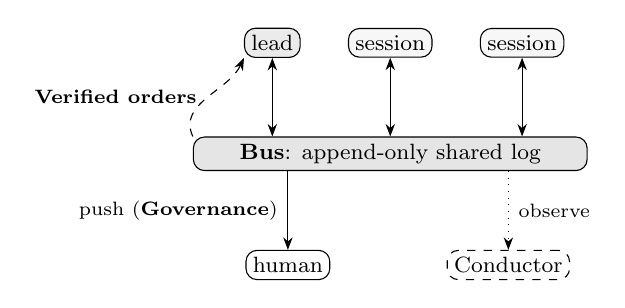
\begin{tikzpicture}[
  font=\footnotesize, >={Stealth[length=4.5pt]},
  every node/.style={inner sep=2.5pt},
  b/.style={draw,rounded corners},
]
  \node[b,fill=black!8] (s1) {lead};
  \node[b,fill=black!3,right=6mm of s1] (s2) {session};
  \node[b,fill=black!3,right=6mm of s2] (s3) {session};
  \node[b,fill=black!10,minimum width=50mm,below=10mm of s2] (bus) {\textbf{Bus}: append-only shared log};
  \draw[<->] (s1) -- (bus.north-|s1);
  \draw[<->] (s2) -- (bus.north);
  \draw[<->] (s3) -- (bus.north-|s3);
  % verified-order loop, kept inside the column (label to the left of the curve)
  \draw[->,dashed] (bus.north west) to[out=115,in=-115] node[left=1pt]{\scriptsize\textbf{Verified orders}} (s1.south west);
  % human gate, left of centre below the bus
  \node[b,below=10mm of bus.south,xshift=-13mm] (hum) {human};
  \draw[->] (bus.south-|hum) -- node[left=1pt]{\scriptsize push (\textbf{Governance})} (hum);
  % read-only observer, right of centre below the bus
  \node[b,dashed,below=10mm of bus.south,xshift=15mm] (obs) {Conductor};
  \draw[dotted,->] (bus.south-|obs) -- node[right=1pt]{\scriptsize observe} (obs);
\end{tikzpicture}
\caption{The composition: persistent \emph{sessions} post to and read an append-only \textbf{Bus}; a
lead fans work as \textbf{Verified orders} (\texttt{deliver} reads the artifact back before
acknowledging); the \emph{human} gates only irreversible acts (\textbf{Governance}: the SHA-pinned push
gate); \emph{Conductor} observes read-only and never drives the agents. The through-line: \emph{verify
the outcome, not the intention.}}
\label{fig:arch}
\end{figure}

\begin{itemize}
\item Bus --- append-only shared log; directed mail is auto-delivered (idle
  recipient woken), which is the courier-elimination mechanism (and an
  \emph{unreliable} one --- \S V-A).
\item Verified orders --- \texttt{deliver} reads the artifact back and refuses unless
  it landed.
\item Project layer --- a nominated lead drafts a job-DAG plan the human approves at
  one gate, then fans jobs (directed orders) along dependency edges; a \emph{peer}, not the
  lead, accepts the lead's own deliverables.
\item Decision shield --- worker decides technical calls and logs them; lead decides
  project calls; a denylist + severity hatch go straight to the human, and the lead is
  \emph{structurally barred} from deciding them.
\item Governance --- SHA-pinned push gate; observer-owned admission throttle (not the
  lead --- fox/henhouse); a measured per-project token meter (estimation is theater;
  only the live meter gates).
\end{itemize}

The through-line is \emph{verify the outcome, not the intention}.

\section{The Method: In-Vivo Adversarial Co-Design}
The design loop that produced the above: (1) a session hits a \emph{silent-loss} failure in
real work (a tool reports success while something is quietly wrong); (2) it publishes the
specimen to the bus; (3) context-divergent peers attack the proposed fix from different
empirical vantages (their histories genuinely differ); (4) the human gates only the irreversible.
Their independence is only \emph{relative to} that divergence --- not one model echoing itself,
but not uncorrelated errors either; bounded in \S V-D.

The loop's \emph{shape} is deliberately unoriginal and we claim no novelty for it: operating a
system to learn what it should have required is evolutionary prototyping
\cite{floyd1984,davis1992}, the spiral model \cite{boehm1988}, and game-day/chaos-engineering
practice \cite{basiri2016}. One post-corpus exercise (2026-08-05, outside the stamp) cuts against
the usual prototyping argument: the first live run of a newly-shipped fleet wind-down protocol,
across 31 sessions, surfaced two silent-success root causes, both in taxonomy class~2 (\S V-B) and
both violating the architecture's own through-line, \emph{verify the outcome, not the intention}
(\S III). The instructive part is not that the drill found them but that \textbf{the requirement
they violate was already published in our own record months earlier} and simply not enforced on a
later actuator. The gap was \textbf{compliance, not knowledge} --- weaker and more useful than
requirements-unknowability: a through-line stated once does not propagate itself to each new
actuator, and the drill is what detects the drift.

\section{Evaluation}
A note on names: throughout the evaluation, a codename in parentheses (e.g.\ \texttt{net-emu},
\texttt{perf-A}) identifies an \emph{individual Claude Code session} --- the participant that
produced, or is the subject of, the adjacent claim. These codenames are role-hinting pseudonyms for
publication, and the artifact package preserves the real$\leftrightarrow$pseudonym mapping. Every quantitative
claim below carries an explicit \emph{provenance tier}; the fleet adopted these as
a discipline and we define them once here (Table~\ref{tab:prov}). The rule the deployment enforces on
itself: a derived or recalled number may never be reported bare, and a claim a reviewer cannot resolve
is, at that moment, not yet evidence.

\begin{table}[t]
\centering\footnotesize
\caption{Provenance tiers used throughout the evaluation.}
\label{tab:prov}
\begin{tabular}{@{}l p{0.60\columnwidth}@{}}
\toprule
Tier & Meaning \\
\midrule
MEASURED & ran it on a censused system, with a resolvable receipt (commit/log) \\
RECALLED & from memory/narration; may be wrong, flagged as such \\
GAP & the honest absence of a measurement we would want \\
LANDED & a mechanism shipped and is live in the running system \\
NULL & a pre-registered test whose falsifier fired (reported as such) \\
reproducible-in-principle & a recipe that outlives the record but has not been re-executed \\
\bottomrule
\end{tabular}
\end{table}

\emph{Corpus, MEASURED from git + bus + \texttt{history.jsonl}, as-of 2026-07-31} (every
count carries this stamp --- the log is append-only and non-stationary, so a
bare number is under-specified; events after the stamp are reported as dated addenda and are
\emph{never} counted, in either direction): 290 commits (38 of type \texttt{fix}); 52 version landings;
2,744 bus messages, of which 2,739 are non-system, from 56 senders
(1,109 directed + 1,107 broadcast + 521 announcement + 2 unclassified $=$ 2,739; directed share
1,109/2,739 $=$ 40.5\%);
6,358 human prompts across 47 projects back to 2026-01-14. \textbf{Division of labour is
spread but with a real head, not a power law} --- the concentration computed by the harvester
(\texttt{evidence-harvest.py} \texttt{\_concentration}), the addressing classified from the same log,
over \emph{all} non-system senders:
Gini 0.698, top sender 9.4\%, top-3 25.4\%, and 13 of 56 senders to reach 80\%.
Many peers carry load, no single dominant author, but a genuine concentration we report rather than
round off to ``distributed.'' Reflexivity confound --- controlled, not just conceded.
Because 196 of the 2,739 non-system messages are this paper's own review/ablation traffic, a
concentration statistic over the whole log could be an artifact of the act of measuring. We therefore
recompute it \emph{restricting to} messages before the paper effort began
(2026-07-24; $n{=}2{,}543$ non-system messages, 52 senders): Gini $0.693$, top sender 9.4\%,
top-3 26.4\%, 13 of 52 senders to 80\% --- \emph{indistinguishable} from the full-log figures above
(Gini $0.693$ vs.\ $0.698$; top-3 26.4\% vs.\ 25.4\%). The head is a property of the \emph{organic}
deployment, not of the paper's own threads; the reflexivity we flag elsewhere does \emph{not}
contaminate this result (both numbers are shown).
Why roles emerged at all --- no one assigned them. Specialization was not designed; it is an
attractor of two forces the substrate creates. Continuity and ownership: a session that built
a subsystem holds the most context about it, so the cheapest place to route the next related task is
that same session --- and routing it there deepens the advantage, a positive feedback that concentrates
each domain onto whoever first worked it. Repeated exposure then hardens it: memory and the bus
make yesterday's work legible today, so a returning session resumes its domain rather than re-learning a
new one. That the resulting head is a \emph{spread} one (Gini 0.698, no dominant author) is because these
forces are \emph{local} --- one attractor per domain --- not because anyone balanced the load. Role
identity is an emergent property of continuity-plus-routing, not an org chart --- which is why it is the
foundation the later findings rest on rather than a policy that could be tuned away.

\subsection{RQ1 --- Courier elimination: a claim we withdraw, and the class it belongs to}
\label{sec:rq1}
\textbf{We do not claim this result.} We report it because the way it failed is a specimen of the
taxonomy in \S V-B, found in our own headline measurement, by a third party, after we considered the
paper ready --- and because the alternative, burying it in threats to validity, would model exactly
the behaviour this paper argues against. The original argument and its evidence follow, then the
defect.


1,109 directed messages (as-of the corpus stamp) are \emph{candidates} for auto-delivery ---
hand-offs a human would otherwise relay --- so the count is a ceiling on relays avoided,
not a claim that all were delivered: the realized count is a \textbf{GAP} --- auto-delivery is a
runtime event the bus log does not record. Indeed the mechanism
is unreliable: in this paper's own production, a directed job failed to auto-wake its peer (stale
watermark) and the human relayed it --- an actual delivery below the ceiling. We report the
counterexample. A second, larger one is dated, outside the stamp: during a post-corpus fleet
exercise (2026-08-05) two independent silent-success defects were live at once --- window-actuation
tools that print their failure to stderr and exit \texttt{0}, and an acknowledgment routine that
terminated before writing its record (\S V-C addendum) --- and the human resumed relaying, driving
the registered fleet through the shutdown by hand, \textbf{while every actuator-level signal
reported success}. This bound is distinct from the GAP above: unrecorded delivery leaves the
measurement \emph{thinned}, whereas an actuator asserting a success that did not occur leaves it
\emph{false}, invisible from inside the measurement. A surfaced reachability check was added in
response (pinned in the replication package). The correct human-touch
instrument is \texttt{history.jsonl} (un-swept, back to January), \emph{not}
transcripts (a 30-day cleanup horizon, \S VII) which also carry an 11.9$\times$
\texttt{tool\_result} overcount trap.

The longitudinal human-touch series (the method's clearest observational signal).
From \texttt{history.jsonl} (human prompts only, un-swept back to January), we normalize touches by
\emph{active project} per month (Table~\ref{tab:touch}). Three monthly buckets cannot
establish a trend, and the middle is non-monotonic (June $\approx$ May), so we report the \emph{shape},
not a single ratio: prompts per active project sit near 70 across May--June, then drop to 36 in
July, \emph{while} concurrent projects grow from 16 to 35 (April, the substrate's build-out month, is
excluded as bootstrap-heavy, as January and March are). To check whether July's drop is a trend or a
single step, a finer weekly breakdown (14 weeks, replication package) shows the same downward
\emph{direction} --- from the $\sim$35--40 band in early May to the $\sim$13 band by late July --- so
we read it as a sustained decline, not a one-month artifact. The weekly and monthly figures
are on different time bases and are not comparable in magnitude: a week's prompt count (roughly a
quarter of a month's) is divided by that week's active projects, so weekly per-project figures run
lower --- the smaller numerator dominates. We use the weekly series only to confirm \emph{direction},
not to sharpen the ratio. This is the one longitudinal signal that speaks to the
\emph{method} claim rather than the compounding claim: as the substrate matures and carries more work
in parallel, the human's per-project involvement drops, which is the courier $\rightarrow$ architect
shift the method is for. The timeline (MEASURED, bus log + git) supports reading this as substrate-driven: the build-out began in
April (the shared bus opened mid-April), and the higher-order primitives that most reduce human
relaying --- auto-delivery, verified orders, the project layer --- landed incrementally and clustered
in July, coincident with July's sharper drop; the decline tracks that ongoing hardening, not a one-time
event (still temporal correlation, not proof). The leverage is larger than the per-project figure alone suggests:
\textbf{from May to July the human took on 2.2$\times$ the concurrent projects (16 $\rightarrow$ 35) for
only $\sim$14\% more total prompting} (1{,}117 $\rightarrow$ 1{,}270 prompts) --- per-project attention
halved while total attention barely moved. At May's $\sim$70-prompts-per-project rate, July's 35
projects would have cost $\sim$2{,}450 prompts; the human spent 1{,}270, the budget for roughly
\emph{half} that many projects. We report it with the standard longitudinal confounds --- the task mix
changed, the operator learned, later projects may be individually smaller, and per-\emph{active}-project
is a proxy for per-\emph{delivered}-project --- so it is a trend, not a controlled measurement.

Who originates the coordination? A direct decomposition, answering the sharpest objection ---
that the human is the real router. We categorized every bus sender (MEASURED,
\texttt{human\_fleet\_decomposition.md}) as human (\texttt{[operator]}, the tag Conductor
posts under when Kyle drives the bus by hand), automated (\texttt{[system]}/watchdog/broker),
or fleet (a Claude session). The human authored 0.9\% of all coordination messages
(26 of 2{,}744) and 1.9\% of the \emph{directed} routing mail (21 of 1{,}109); the fleet
authored 95.5\% and automated/system senders the rest, so \textbf{over 99\% of coordination
originates from non-human senders}. And that fleet coordination is load-shared, not funneled through a
lead: among the 52 fleet senders the busiest is 9.8\% of fleet mail, the top three 26.6\% (fleet-only
denominator, so slightly above the 25.4\% all-sender figure above), and it
takes 7 to reach half --- there is no human-proxy hub routing the traffic. The honest limit:
the bus is the Claude$\leftrightarrow$Claude channel \emph{by construction}, so this bounds the human's
share of the \emph{shared} channel, not the prompt channel above --- but the two agree, and that is the
point: $<$1\% of bus traffic \emph{and} a falling per-project prompt intensity both point away from a
human doing the routing. What the human owns --- goals, framing, the irreversibility gate --- is
architect work, not courier work, which is precisely the claim.

And RQ1 is a \emph{tradeoff}, not a pure win. Coordination over an async bus + a lead's wake cycle can be slower in
wall-clock than a synchronous human courier: in this deployment a directed wake took
minutes, and in the counterexample above the mechanism failed outright and the human
was faster. The substrate optimizes the human's attention (fewer relays to run), and
can \emph{worsen} the critical-path latency of any single hand-off. The honest claim
is \emph{attention saved}, not \emph{time saved} --- RQ5 (\S V-E) shows the same shape at the
single-agent level (context bought steps and wall-clock but \emph{more} tokens).

\subsubsection*{The defect, and why it is fatal rather than a caveat}
The instrument is \texttt{history.jsonl}, which records human prompts. It loses records. The
mechanism was found by reading the writer rather than by auditing the data: a file lock is attempted
and, after a bounded number of failures, silently abandoned --- the write is dropped with no error,
no retry and no marker. Contention rises with the number of concurrently active sessions, so
\textbf{the loss is concentrated rather than random, and it scales with fleet size.}

That is the same direction as the claimed effect. Our claim was that human touch per active project
\emph{falls} as concurrent projects \emph{rise}; the instrument drops more records exactly as
concurrency rises. A decline would therefore appear in this measurement whether or not one occurred.
This is not a limitation to disclose alongside the result --- it is a mechanism that can manufacture
the entire result, and it runs in the direction that flatters the paper's thesis.

\textbf{It is class-2 in \S V-B's terms: informative missingness.} The taxonomy already names the
shape --- a monitoring mechanism whose failures concentrate on the cases satisfying the condition it
certifies, so the census is \emph{biased, not merely thinned}. We wrote that class from the
acknowledgment-routine defect (\S V-C addendum) and did not apply it to the measurement three
subsections earlier. \emph{Knowing the class did not protect the author who wrote it.}

Two further properties make it a good specimen rather than merely an error. It is \textbf{silent}:
no count is implausible, no arithmetic fails, and every figure in Table~\ref{tab:touch} is internally
consistent. And it is \textbf{invisible from inside the measurement}: no analysis of
\texttt{history.jsonl} can detect records that were never written --- only reading the writer can,
which is what happened. A completeness check requires a second, independent enumeration, and we had
none.

\textbf{What we would need to claim it.} An independent record of human prompts --- a
terminal-level capture, or a writer whose dropped writes are counted rather than discarded --- and a
re-measurement against it. We did not have one, and we do not report the effect. The counting
machinery remains in the replication package so a future measurement can be compared against it.

\subsection{RQ2 --- Failure modes closed, with real ablations (+ the defect taxonomy)}
\textbf{MEASURED}: of the 38 \texttt{fix} commits (as-of the corpus stamp), $\sim$20 close \emph{named coordination failure modes}.
Several are ablation-structured --- disable the mechanism, the failure returns --- and
at least one ablation \emph{ran in operation}: the SHA-pinned push token, unpinned, would let
an approval for commit A push commit B; the gate refused a stale approval live during
this project. The two-phase-commit and member-cursor ablations are specified and pending.

A defect taxonomy the fleet converged on (a secondary contribution). Writing and
ablating the cases surfaced a small, reusable classification of the \emph{silent} defects the
method exists to catch, each with a distinct remedy --- the point being that a single
discipline (``just replicate,'' ``just tag'') sails past most of them:

\begin{enumerate}
\item Single sample promoted to a property --- a condition true of one run asserted as
  general. Remedy: replicate + tag. Sharpened (perf-A): a \emph{measured} number
  promoted past its conditions is \emph{worse} than a derived one, because the \texttt{measured}
  badge actively defends the error.
\item Green-but-wrong / wired-but-broken in the untested direction --- a gate green +
  documented + shipped, passing every gate-ON test while the gate-OFF path leaks (emu-C,
  net-emu). Replaying the green measurement \emph{n} times passes \emph{n} times; the only fix
  is asserting a different measurement --- execute the off-state / your own
  reproduction once.
  A post-corpus specimen adds an axis: the untested direction can be \textbf{selected by the very
  condition the mechanism exists to attest}. The acknowledgment routine of \S V-C's addendum
  reached its fatal path only when a session had \emph{exactly zero} unpushed commits, so failure
  concentrated on sessions satisfying the very condition the ack certifies --- \textbf{informative
  missingness} (MNAR, \cite{rubin1976}) in a monitoring mechanism, so the census is \emph{biased},
  not merely thinned. Here the class-2 remedy is necessary but insufficient: \textbf{zero unpushed
  is not the off-state; it is the attested value, on the nominal success path} (the off-state, a
  dirty tree, \emph{was} exercised), so the remedy extends to the boundary value of the predicate
  the mechanism selects on.
\item Provenance-tier silently dropped during remediation --- re-anchoring a number to
  a \emph{recipe} downgrades MEASURED $\rightarrow$ reproducible-in-principle until someone runs
  it (band, emu-C). Remedy: run the recipe and \emph{say you did} (emu-C did --- the
  mutation reproduces \texttt{1,409,307,648}).
\item Conservative-error-is-durable --- a wrong-but-safe-looking value evades the
  provenance check that would normally catch it. ``A conservative error is not a safe error; it
  is a durable one.''
\item Thoroughness regression --- the context shortcut that made the agent fast made
  it skip the secondary gap (mcu-emu DISMAP; perf-B's third site). Remedy: re-derive under a
  differently-drawn boundary / forced first-principles trace.
\end{enumerate}

And the remedy split the same convergence produced: TAG (cheap disclosure;
catches a condition you measured but did not state) $\rightarrow$ ABLATE (an
invariant/control; catches a condition you \emph{believed held and did not}) $\rightarrow$
HARVEST (a parallel peer at the same boundary building the same artifact is a
\emph{naturally-occurring} off-state ablation --- emu-C$\leftrightarrow$emu-B,
perf-A$\leftrightarrow$perf-B --- cheaper than a designed one, and record-visible: cross-tree
agreement on different fixes is derived-not-copied). \emph{Shipping only the tag documents the
bug rather than fixing it.}

\subsection{RQ3 --- Defect discovery by vantage (machine-evidenced)}
We split two claims review conflated. (i) A measurement vantage exists (supporting,
not the RQ3 claim): MEASURED (build-A), a 38-Bash-call build had 17 measurement calls (12
\texttt{/proc} probes, 4 runs) --- a vantage a browser assistant could not occupy, proven from
the event log. (ii) A peer caught what the author shipped (the actual RQ3 claim, and
it needs the \emph{same} timestamp rigor --- A ships at t0, B refutes at t1, both from the
record). We enumerate the record-attested cross-session catches (14 attested, 13 classifiable; tabulated in
the replication package) and here name four representative ones, each with \emph{attribution
corrected} against the record after review flagged two mis-attributions in earlier drafts (a
``\texttt{api-svc} tag-flip caught by a peer'' was in fact self-caught, and a claimed ``slam-A
caught four errors'' had no record --- both removed).
image-gen $\rightarrow$ api-svc: api-svc's RTX-5090 idle-power \emph{denominator}
(64.97~W) was contaminated by image-gen's own resident tenant; a clean board idles near 21~W, a
physical floor image-gen held.
doc-A $\rightarrow$ slam-A: slam-A's ``fixed-K Amdahl overhead'' bandwidth model,
refuted by diffing two derivations on the shared tensor table (K doubles when the workload doubles,
so a fixed overhead is impossible --- the model refuted itself on its own arithmetic).
media-npu $\rightarrow$ socdev-A: socdev-A's ``verified'' NPU INT8 model was
quantized \emph{without calibration normalization} (wrong input scale); media-npu reproduced its
exact numbers to five decimals, then corrected the parameter.
bench-A $\leftrightarrow$ net-emu: bench-A's ``+64~s rejoin stall'' was its own scorer's
arrival-stamp backlog --- net-emu relocated the measurement \emph{into the guest} (a guest-emitted
timestamp bench-A structurally cannot make; a pinned commit in the replication package) and a subsequent scorer
replay put guest-side re-acquisition at 0.0~s. We keep the two artifacts distinct (the instrument
commit vs.\ the replayed figure), pinned t0 (stall reported) $<$ t1 (refuted).
A record-attested instance from the ablations: in \texttt{ablation\_perf-A} a blind,
zero-context arm caught a real overstatement in the author's own case (129 defective cells
reachable via the engine API but \emph{not} the shipped UI) in nine tool calls. \textbf{Cases are illustration; the events (order claims,
timestamps, tool-call logs) are the evidence.}

\textbf{Post-corpus addendum} (2026-08-05, outside the as-of stamp; \emph{not} counted in the
14/13 above). The catches above are peers refuting a peer's technical \emph{result}; this one
differs in kind --- the defective artifact was the \textbf{coordination substrate itself} and the
catching vantage was \emph{being subject to it}, so it supports the \S V-D bound rather than
incrementing it. \emph{Disclosure, load-bearing here:} \texttt{substrate-dev} below authored the
wind-down machinery \textbf{and drafted this paper}; the catch is reported against ourselves.
All five events are timestamped in the append-only record --- \textbf{four on the bus, one in git}
--- on one day. \textbf{11:34:25}: \texttt{mcu-emu}, winding itself down, publishes the root cause
of an acknowledgment routine that wrote no record --- a counter that prints \texttt{0} and
\emph{exits non-zero}, terminating the routine under \texttt{set -e}. \textbf{14:32:54}:
\texttt{substrate-dev} commits a fix for a \emph{different} defect in the same routine.
\textbf{17:17:25}: it broadcasts to the fleet that the bug is fixed. \textbf{17:20:53}
(\textbf{3m28s later}): \texttt{band} measures the shipped routine from a clean tree --- no
output, exit 1, no record written. \textbf{18:09:05}: \texttt{band} publishes an audit enumerating
\textbf{7 acknowledged against 24 not} (31 registered tags). Both commits are pinned in the
replication package.
We record it in \textbf{both} directions. As a vantage instance it is strong --- the refutation came
from \emph{operating} the mechanism, timestamped against \texttt{substrate-dev}'s own claim. As a
\textbf{substrate failure} it is equally real: the refutation sat on the bus \textbf{at least
5h43m} before the broadcast, so the delivery machinery this paper evaluates never put it in front
of the session that authored the claim. \textbf{A vantage published but not \emph{consumed} is a
bound on the substrate, not only a credit to the peer.} The episode is a class-3 instance of our own taxonomy
(\S V-B), violating a remedy we had published; being \textbf{empirical-vantage} --- a measured
exit status, not a same-input reasoning disagreement --- it leaves \S V-D's
no-same-input-reasoning-catch statement \textbf{unaffected}.

\subsection{RQ4 --- Compounding capability: withdrawn, and why it could not be retested here}
We set out to show that a session carrying lived context solves what a fresh one cannot. An earlier
draft reported the negative --- that it does not --- and called it the paper's most solid evaluated
result. \textbf{We withdraw both the claim and the negative.} The study could not detect the effect
whose absence it reported, for two independent reasons, each verified against our own artifacts after
an adversarial review raised them.

\textbf{The ablation never manipulated the construct it named.} The text described ``a genuinely
isolated fresh session versus a context-carrying one.'' The ablation record shows \emph{both arms
were fresh memoryless subagents}, differing only by a hand-distilled summary placed in the prompt.
What was refuted, therefore, is that a summary injected into a prompt helps --- a different and much
weaker proposition. No arm of any ablation ever ran a live context-carrying session against a fresh
one.

\textbf{And the falsifier was unreachable.} Across six ablations and the baseline, \emph{no arm of
any task ever failed}. A design whose falsifier requires the fresh arm to fail cannot fire on tasks
nobody fails; the uniform success is a ceiling effect, not a null.

\subsubsection*{The replacement, and the limit that stopped it}
We pre-registered a corrected experiment before running anything: fixed $N$, interleaved arms,
isolation established by construction and transcript audit rather than self-report, a rubric hashed
with the file, and grading by a session that authored neither the code under test nor the
registration. It was witnessed by non-authors, amended three times pre-results in response to their
objections, and every amendment is a pure append --- the registered text is byte-identical under
every later revision.

It has not run, and on this deployment it cannot. A qualifying task must have a live
context-carrying arm with genuine domain history, at the registered $N$. \textbf{This fleet runs one
session per repository}, so the only domain that can supply that many live arms is the one the
authors wrote --- which fails the registration's own author-circularity criterion. Three candidate
tasks were nominated and disqualified for three structurally different reasons (access, cheap
re-derivation, and author-circularity); the constraint is not candidate quality.

The registration committed in advance to how this outcome is read, precisely because it flatters a
reframe we were separately considering: \emph{inability to construct a discriminating task is
reported as a measurement-capability limit of the deployment, and never as support for the
negative.} We report it as that. The generalisable form is a property of the architecture rather
than of the hypothesis: \textbf{a one-session-per-repository fleet cannot furnish a within-domain
control arm for any claim about accumulated context}, because the only session with the history is
the only session there is.

\subsection{RQ5 --- Baseline: reported, not claimed}
We pre-registered and ran one matched task both ways: a fresh memoryless session against the peer
with the most lived history in the target file, both from an identical repo copy, graded on six
behaviours by a black-box acceptance test, with the directional prediction committed before either
arm ran and the instrument first proven satisfiable against an unmodified baseline.

\textbf{The design stands; the target did not.} Review established that the file chosen as ``the
peer's most lived history'' was roughly one day old at baseline. Whatever the arms differed in, it
was not accumulated context --- it was authorship recency, which is a different variable with a
different meaning. We therefore report the experiment and not its outcome.

We keep it here for two reasons. The apparatus is reusable and is pinned in the replication package
--- a later study with a correctly aged target can run it unchanged. And the failure is itself a
member of \S V-B's taxonomy: a pre-registered experiment, correctly executed, measuring a quantity
other than the one its variable was named for. Pre-registration constrains \emph{analysis}; it does
not verify that the independent variable is the construct.

\subsection{The paper as an instrument (an operational finding, not a controlled result)}
Asking sessions to substantiate claims \emph{to an external audience} forced verification of
things taken on trust internally. In git: \texttt{perf-A} found a 46-day defect (129 cells
rendering wrong fps, count never zero, never visible) while writing its case --- after 46 days of
use/test/review found nothing; \texttt{perf-B} surfaced a validation-across-an-unsafe-version
provenance defect the same way. We state the hit-rate: of 19 case-writing sessions,
4 ($\sim$21\%) reported a correction surfaced during the writing (\texttt{perf-A},
\texttt{perf-B}, \texttt{meter-A}, the RQ5 apparatus's own frozen-test defect); the rest
reported none. We are careful about what this is and is not. It has no control arm: we did
not measure how many defects surface in 19 sessions of \emph{equivalent effort spent not writing for
an external audience}, so 21\% has nothing to beat, and the underlying effect --- careful explanation
to an outside reader surfaces latent defects --- is well established for design documents and code
review; \emph{the only novel element here is that the writers were agents}. And it is not fully
``testimony-free'': the \emph{commits} are machine evidence, but the \emph{attribution} (``the defect
was surfaced by the act of writing'') is a causal judgment made and reported by the same sessions ---
two different epistemic objects, which we keep separate. So we report it as an \textbf{unanticipated
operational finding with a stated hit-rate and no control arm} --- worth recording, not a headline
result.

\section{Implications for Practitioners}
The measured results reduce to four working rules; each carries the bounds of \S VII.

\textbf{1. Fund the carrier, not the session.} Effort that moves knowledge into the committed,
executable carrier --- code, asserts, invariants, checked-in operating docs --- buys
capability: a fresh clone holding it reached every fix we tested (\S V-D, \S V-E) --- though
note that \emph{every} arm succeeded, so this is measured where capability was never the binding
constraint. Effort that preserves session memory buys speed, not correctness, \emph{on tasks of
that kind}. When the two compete for budget, the
carrier wins.

\textbf{2. Route on demonstrated history --- and audit the sessions you route to.} A lead can route
work by what a peer has actually done rather than by a declared role, and that is what the record
supports. \emph{We no longer quote an efficiency figure for it:} our matched-task numbers came from
the baseline whose target proved a day old (\S V-E), so they measure authorship recency, not
accumulated context. But context also
produced the one failure class unique to it: the \emph{thoroughness regression}, in which a
context-carrying session pattern-matched a staged answer and stopped short of the second defect
a blind arm caught (\S V-D). Long-lived sessions therefore need a periodic fresh-eyes pass ---
a blind clone on the same task --- as a standing control.

\textbf{3. Write fixes into the executable carrier, not into prose.} The stale-doc ablation
found a wrong prose carrier to be ``neither the asset nor the liability'': every arm detected
the staleness against the code (\S V-D). Prose narrates; code, tests, and invariants govern. A
fix that exists only as narration has not compounded.

\textbf{4. Copy the cheap primitives first.} The substrate's load-bearing mechanisms ---
verified orders that read the artifact back before acknowledging, SHA-pinned approval tokens,
an observer-owned admission throttle --- are small, model-agnostic, and follow one rule:
\emph{verify the outcome, not the intention} (\S III). They transfer whether or not one adopts
the fleet.

\section{Threats to Validity}
\begin{itemize}
\item Self-evidencing circularity. A corpus of first-person cases
  about coordination, curated for a paper about coordination, is self-report at scale.
  Mitigation: cases are demoted to illustration; every load-bearing claim rests on the
  mechanical record.
\item Single-model confound. Divergence is memory/context, not different minds; we own
  the composition and do not claim emergence.
\item Selection bias / no denominator. The open call collects confirming specimens by
  construction. We hold $\geq$1 deliberate counter-case (a bug recognized instantly but
  re-tripped twice --- recognition cost $\rightarrow$0, prevention cost unchanged), frame the
  corpus as illustrative, and note the missing denominator explicitly.
\item 30-day record horizon. The platform silently deleted transcripts $>$30 days (now
  disabled); the pre-June transcript record is GAP. Longitudinal claims use \texttt{history.jsonl}
  + git, which survive.
\item Ablation methodology. (a) \emph{Grading
  asymmetry} --- two of six ablations (\texttt{perf-A} and the C2 sequel) published a rubric hash
  \emph{before} results; the other four are honestly-run but post-hoc graded, so
  retrofitting is disavowed, not detectable. \texttt{perf-A} is the \emph{only} ablation whose
  both arms ran under a pre-published rubric; C2's pre-registration covers its rubric and
  its fresh (Arm~B) runs, but its Arm~A was scored post-hoc from record ((c) below), so C2 sits
  partly in both categories. (b) \emph{Isolation is a claim, not a given} --- the
  harness pre-injects a fresh agent's cwd, git status, and memory \emph{index}, so ``blind'' arms
  are mitigated, not sterile; the cleanest arms used fictional subjects (emu-B) or
  audited each agent's actual tool calls. (c) \emph{Historical arms are not re-runnable} --- some
  context-carrying arms (the INT8 ablation's Arm~A and C2's Arm~A) are transcripts of past work
  (the answer already known), so they bound
  rather than measure. (d) \emph{N is small} (1--8/arm) and outcomes are often categorical (no
  variance). Each is stated in the individual \texttt{ablation\_*.md}.
\item $N{=}1$, one operator, one workstation, one model family.
\item Self-authorship, including \emph{this reframe} --- written by an interested lead who is
  also the author of the substrate under evaluation (\S V-C addendum),
  corrected by peers. We prefer machine evidence throughout; the \textsc{recalled} tier is defined in Table~\ref{tab:prov} and \emph{is applied nowhere in this paper}, which is the honest report --- an earlier draft promised the tag and used it once, on a claim now withdrawn. A provenance tier that is never applied is a tier the reader should not be asked to trust in.
\item The bystander-catch corpus contracted under audit. While preparing this paper, two
  claimed cross-session catches did not survive record-checking --- a ``\texttt{api-svc} tag-flip
  caught by a peer'' was in fact self-caught, and ``slam-A caught four independent errors'' had no
  case-file or bus record --- and both were removed (\S V-C). We report the contraction rather than
  quietly correcting it, because it is itself evidence for the provenance discipline the paper claims:
  the corpus is what the record supports (14 attested, 13 classifiable), not what narration remembered.
\end{itemize}

\section{Future Work: A Pre-Registered Replication}
The paper's central threat is $N{=}1$ --- one domain (systems/tooling), one operator, one
workstation, one model family. We therefore \emph{pre-register} the replication that would
falsify or corroborate the claims, and state its prediction before running it (predict-then-run,
a discipline the fleet itself enforces):

\begin{itemize}
\item Vary the confounding axes, not the surface. Repeat the experiment on a
  structurally different domain --- ideally not software (e.g.\ scientific literature
  synthesis, hardware/product design, operations, or creative work), where ``a task'' and
  ``expertise'' mean something different in kind. Ideally with a different human
  architect, to remove the ``maybe it is this operator'' confound.
\item Hold the \emph{method} constant, vary the \emph{content}. The claim under test is
  not ``the tool runs on another codebase'' but that \emph{the composition} --- persistent
  context-heavy peers + a shared bus + verified orders + a human gating irreversibility ---
  reproduces the signatures: compounding competence (a measured downward per-task-cost
  trajectory via the same ablation protocol), peer review catching the lead's blind
  spot, and the self-designed substrate --- and, per the \S V-D conjecture, whether
  accumulated context confers an advantage in task origination, the step our ablations held fixed.
\item Prediction (falsifiable): if the principles are real and not artifacts of this
  domain/operator, the \emph{same} signatures appear on the new ``thing''; if they are artifacts,
  they do not. A null result is as informative as a positive one and will be reported as such.
\item Feasibility: the replication needs no new system --- only a new \emph{goal}
  pointed at a fleet (\texttt{project new <thing>}), which is precisely what makes the method's
  claim to generality testable rather than rhetorical.
\end{itemize}

This is the sequel experiment; naming it here is the honest acknowledgement that a single
deployment, however rich, establishes a \emph{method worth replicating}, not a law.

\section{Conclusion}
Conductor is an experience report on a nameable composition --- one model, durable per-session
memory, a shared bus, a human gating only irreversibility --- that co-designed and hardened its
own coordination substrate in vivo. Its headline intuition --- that accumulated context makes a session more capable --- we could not
test. An earlier version reported that it does not hold; we withdraw that, because the ablation
behind it never varied the construct it named and its falsifier could never fire. The corrected
experiment is pre-registered and witnessed and \emph{cannot be run on this deployment at all}: a
fleet with one session per repository has no second session carrying the same history.

What the deployment does establish is smaller and sturdier. Silent coordination defects fall into a
small number of classes with distinct remedies, and we name them. Peers with different vantages catch
what an author and an operator miss --- including, repeatedly, in this paper: three of the claims
above were withdrawn on defects found by other sessions and an outside reviewer after we thought the
work was finished, and every one of those defects ran in the direction that flattered us. The process
that produced those corrections --- peers refuting the lead on the record, an ablation refuting its
own author --- is the mechanism under study, and it is the part we would carry to another
deployment.

The reusable contribution is the method: in-vivo adversarial co-design by persistent,
context-divergent peers under a reversibility-gating human, offered as an existence proof with
a stated mechanism, not a validated superiority. Its cleanest demonstration is this paper's own
review. The internal panel, at the deployment vantage, caught substance --- a circularity, a
single-model confound, unrun ablations; independent external review, at the submission vantage,
caught what the panel structurally could not --- cross-section consistency, arithmetic, and
venue compliance. Which vantage caught which defect class is checkable in the archived draft
series and the paper's own git history: the vantage bound of \S V-D, one level up.

Three secondary observations travel beyond this deployment: the silent-defect taxonomy and its
TAG$\rightarrow$ABLATE$\rightarrow$HARVEST remedy split (\S V-B); the non-independence
discipline --- before crediting two results as corroboration, check for a shared generative
mechanism, and discount if found (\S V-D); and the durability ladder --- untracked
$\rightarrow$ committed $\rightarrow$ pushed --- because a claim a reviewer cannot resolve is,
at that moment, not yet evidence. The working summary for practitioners is \S VI: fund the
carrier, use sessions for speed and routing, audit for the regression, copy the cheap
primitives.

\section*{Appendix: Evidence vs.\ Illustration}
\textbf{What the replication package can and cannot resolve.} We state this plainly because the
paper sets the bar itself (\S V): \emph{a claim a reviewer cannot resolve is, at that moment, not
yet evidence}. RESOLVABLE: the substrate repository (git history, the \texttt{ablation\_*.md}
files, the pre-registered specs and their hashes, \texttt{history.jsonl}-derived series). \textbf{NOT
RESOLVABLE: the commits backing the RQ3 cross-session catch table.} Those defects were fixed in
separate hardware- and vendor-specific repositories that are not ours to release, so their hashes
do not resolve against the released package. By our own rule the RQ3 corpus is therefore
\emph{attested but not reviewer-checkable}, and we mark it so rather than let a pinned-looking
hash imply otherwise.
\textbf{Evidence (MEASURED):} the mechanical record (git, bus, \texttt{history.jsonl}, spend
meter), the six A/B ablations (the \texttt{ablation\_*.md} files, replication package), and the
pre-registered RQ5 baseline (\texttt{cases\_rq5-baseline.md} plus the frozen spec/test and
both arms' diffs). These carry the headline claims. Illustration (dataset,
not evidence): twenty first-person \texttt{cases\_*.md} specimens (from the 19 case-writing sessions
of \S V-F --- one session contributed two) + the platform specimen
\texttt{cases\_cleanup-timer}, retained to illustrate design patterns, not cited as proof of
any headline claim. Curated to five in-body illustrations, each mapping to a distinct claim:

\begin{enumerate}
\item \texttt{perf-A} --- paper-as-instrument (\S V-F): a 46-day latent defect surfaced \emph{by
  writing the case}, and an ablation that \emph{refuted the author's own Case 2} --- the
  reflexive mechanism at its sharpest.
\item \texttt{net-emu} $\leftrightarrow$ \texttt{bench-A} --- RQ3 bystander/vantage:
  observer-vs-subject mutual correction (bench-A's ``+64 s stall'' was its own backlog;
  net-emu's guest-side clock settled it) --- each catches what the other structurally cannot.
\item \texttt{mcu-emu} (ablation) --- RQ4b: the \emph{thoroughness-regression} specimen (context
  pattern-matched a staged answer and stopped; the blind arm caught the second register class).
\item \texttt{app-A} (a consumer app handling private user data) --- RQ4a convergence: a 5th
  independent derivation of ``the model narrates, deterministic code owns the value'' reached
  \emph{from privacy} --- convergence that survives a change of \emph{force}.
\item \texttt{image-gen} --- lived-expertise routing (\S IV): the GPU-lease-lying / cost-blow-up
  incidents it was assigned to document \emph{because it lived them} --- the motivating case for
  routing on history.
\end{enumerate}

Several cases were corrected during the paper's own writing (perf-A's Case 1 severity
downgraded from user-visible to latent; perf-B's propagated overstatement retracted),
logged as \S V-F specimens.

\section*{Disclosure: Use of Generative AI}
% TODO (final re-stamp, Fable round-4): add ~\cite{claudecode} after "(Anthropic)" below -> becomes
% ref [19]; the staged entry is in references.bib (set its access date).
%
% PAGE BUDGET — ⚠️ REOPENED 2026-08-08 BY THE HONESTY EDITS. ~25 body lines over. DO NOT trim
% these back out; resolve it when the framing is settled (see below).
%   Limit (CONFIRMED, ICSE 2027 SEIP CFP): 10 pages main text + 2 for references. Deadline
%   Fri 23 Oct 2026. It WAS compliant at 10+1 before this round.
%
%   WHY IT REOPENED, and why that is correct: an adversarial PC-style review returned REJECT with
%   one core objection — the study cannot detect the effect it reports the absence of (the
%   load-bearing ablation manipulates a prompt paragraph, not session context; and no arm of any
%   task ever failed, so the dependent variable has zero variance). The fixes that do not require
%   re-running anything are CAVEATS, and caveats cost lines. Applied this round: scope qualifier on
%   the central finding, the touch metric restated as the arithmetic it is, RECALLED finally
%   APPLIED (it had appeared only in its own definition and a promise to use it, while MEASURED
%   appeared 12x), §VI Rule 1 scoped, Table 1's stamp mismatch with its own artifact stated, and a
%   replication-package scope statement admitting the RQ3 commit hashes do not resolve.
%
%   DO NOT PAY FOR THIS OUT OF THE CAVEATS. They are the point. Pay for it after the framing
%   decision, because the leading candidate reframe — promoting §V-D's reproducibility/open-search
%   tension from a subordinate clause to the thesis — rewrites enough of §I and §V-D that trimming
%   now would be wasted work. If the framing stays as-is, the §I Summary-of-findings trim is still
%   unspent and is the designated fallback.
This paper reports on, and was substantially produced by, a fleet of \emph{Claude Code}
(Anthropic) sessions --- the same system the paper studies --- under the human author's direction.
We disclose the division of labour precisely, because for this subject it is itself a finding. The
agent sessions: drafted the prose of every section across the full draft series; \emph{adversarially
peer-reviewed} one another's drafts on the shared bus and produced the three-lens review that forced
the v2 and v4 reframes; designed and executed the six A/B ablations --- two of them (\texttt{perf-A}
and the C2 open-search-ceiling sequel) pre-registered --- and the RQ5
baseline; and mined the git, bus, and \texttt{history.jsonl}
records for the quantitative evidence. The human author set the goal, made every
irreversible decision (each \texttt{git push} was human-gated), chose the framing and the venue,
took final responsibility for every claim, and is the sole party accountable for this submission. No
text was accepted without human review. All quantitative results were re-derived from the primary
records cited. Independent human external review (multiple rounds) then caught defect classes the
fleet's own review structurally could not --- cross-section consistency, arithmetic, and
venue-compliance --- and drove the final revisions; \S IX notes why this split falls out of the
paper's own thesis. Per ACM/IEEE authorship policy, the generative-AI system is \emph{not} an author;
its contribution is disclosed here and acknowledged below.

\section*{Acknowledgment}
The author thanks the Conductor fleet --- the persistent \emph{Claude Code} sessions named
throughout this report --- whose adversarial review, ablations, and
first-person specimens are the substance of this work, and without which neither the system nor
the paper would exist.

% ---- BIBLIOGRAPHY (verified 2026-07-27) ------------------------------
\bibliographystyle{IEEEtran}
\bibliography{references}

\end{document}
